The detection of the MPS stations is an important part at the competition. This chapter gives detailed insights into the newly implemented SmartRobotinoDetection component. 


\subsubsection{Overview}

The SmartRobotinoDetection component has only one task: it shall detect the MPS stations nearby the robot on the field. Therefore, if the component gets triggered, it commands the robot to perform a 360 degree turn and detect all the machines around.

\subsubsection{Old Version 2017}
The former team implemented the SmartMPSDockingRoboCup component. 

\begin{figure}[h]
\centering
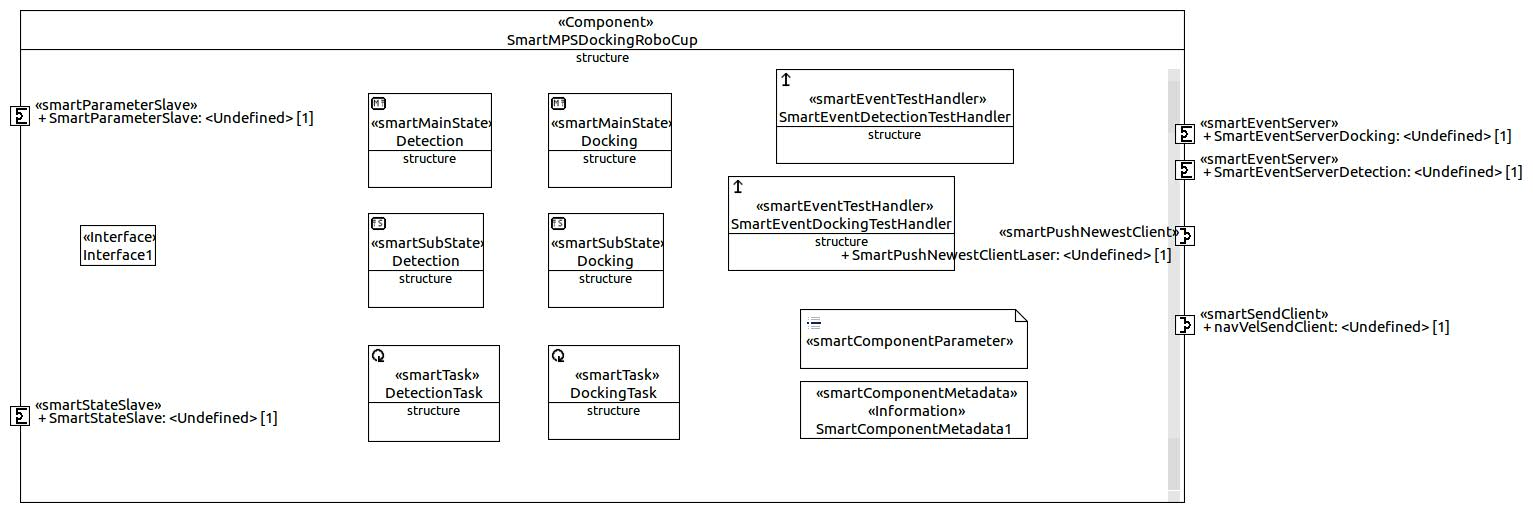
\includegraphics[scale=0.4]{pic/SmartMPSDockingRoboCup.jpg}
\caption{Model of the old MPS Detection/Docking Component}
\label{fig:dockingold_overview}
\end{figure}

Their idea was to combine the detection of the MPS stations and docking to the stations in one component. The detection worked most of the time, but the docking was completely random. This chapter just describes the detection part, and the docking is described in the next chapter. 
The combination of different tasks (detection and docking) contradict the idea of SmartSoft, where separate software components for separate  skills are recommended. By splitting up detection and docking, it would also be possible to replace on the fly the detection via the laser scanner by the detection via the camera, mounted on the robot.
Further the old SmartMPSDockingRoboCup component is implemented in a very confusing way and is hard to understand, so the team of 2018 decided to completely rewrite the component and discard the old one.


\subsubsection{ New Version 2018}

Each Skill component should satisfy one specific task.\\
Therefore the new SmartRobotinoDetection component just detects MPS machines around the robot and the component model is accordingly simple.

\begin{figure}[h]
\centering
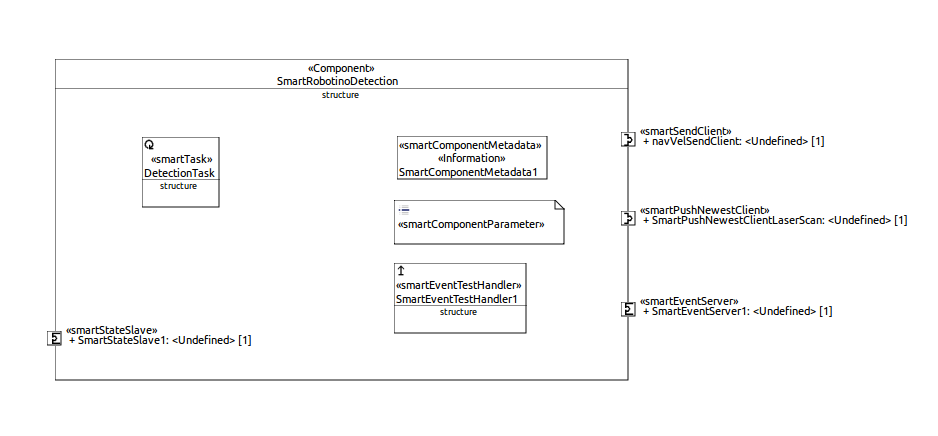
\includegraphics[scale=0.65]{pic/detectionComponent.png}
\caption{Model of new MPS Detection Component}
\label{fig:dockingNew_overview}
\end{figure}

The new detection component consists of one task (e.g. DetectionTask). If this task is triggered, the component commands the robot to perform a 360 degree turn at the current position. Every detected MPS station is sent back to the Sequencer, for further processing. 
The algorithm for the detection of the MPS station is more or less the same like the years before. However, the verification of the detected MPS station changed. The complete boundary of the field is excluded in the new version. Therefore, it is not possible for the robot, to confuse the boundary of the RoboCup field with a MPS machine. This simple approach led to very good testing results. 

\subsubsection{Detection Results}
The results are sent via the CommStationDetectionEventResult object, which contains 

\begin{enumerate}
\item MPSStationDetectionResult
\item CommMPSStationData (as a vector)
\end{enumerate}

The MPSStationDetectionResult is an enum which provides general information whether a MPS was found (MPS\_FOUND) or not (NO\_MPS\_FOUND).
The CommMPSStationData vector is empty if the component did not find any MPS stations. Because the docking algorithm of 2017 was very complicated, lots of information of the MPS station where needed. Thats why the CommMPSStationData contains lots of fields and seems bloated. It contains:

\begin{itemize}
\item orientation1 -> radial orientation corresponding to first docking point
\item orientation2 -> radial orientation corresponding to second docking point
\item centerX -> X coordinate of the MPS center point
\item centerY -> Y coordinate of the MPS center point
\item dockingPosX1 -> X coordinate of the first docking point
\item dockingPosX2 -> X coordinate of the second docking point
\item dockingPosY1 -> Y coordinate of the first docking point
\item dockingPosY2 -> Y coordinate of the second docking point
\item zone -> Zone of the RoboCup map where the MPS resides
\end{itemize}

The new detection component still uses the CommMPSStationData structure. Just the corners of the appropriate stations are relevant and thus most of the other parameters are deprecated. In the future this data structure needs a clean-up. For the new docking algorithm, just the corners of the appropriate stations are relevant, so the detection just writes the first corner in the dockingPosX1 and dockingPosY1. The second corner is written in the dockingPosX2 and dockingPosY2 fields. The rest of the parameters are ignored.

\paragraph{Configuration of the excluded Border} $\;$ \\
The component can exclude the boundary of the field. For this, some smartComponentParameters can be set in the component:
 
\begin{itemize}
\item xMin
\item yMin
\item xMax
\item yMax
\end{itemize}

These just define a rectangular area in world coordinates of the RoboCup coordinate system. Potential machines outside this area are not considered and excluded.
It is necessary to adjust those parameters at the competition, because the RoboCup field is much bigger than the testing field in the laboratory.
To switch the feature off, just set huge numbers for xMax and yMax, and very small numbers for yMin and yMin.







